%%%%%%%%%%%%%%%%%%%%%%%%%%%%%%%%%%%%%%%%%%%%%%%%%%%%%%%%%%%%%%%%%%%%%%%%
%
% Template latex file for a common article class for class notes
% and write ups. Additional Configuration and styling options are 
% commented out. ex. Table of Contents and Title page
% 
% Author: Amy Bui
% 
%%%%%%%%%%%%%%%%%%%%%%%%%%%%%%%%%%%%%%%%%%%%%%%%%%%%%%%%%%%%%%%%%%%%%%%%
 
\documentclass[12pt]{article}
\usepackage[utf8]{inputenc}
\usepackage{parskip}
\usepackage{tabularx}
\usepackage{array}
\usepackage{appendix}
% \usepackage[showframe=true]{geometry}
\usepackage{changepage}
% \usepackage{csvsimple}
% \usepackage[framemethod=tikz]{mdframed}
% \usepackage[color, leftbars]{changebar}
% \usepackage[inkscapeformat=png]{svg}
% \usepackage{svg}
% \usepackage[inkscape={/Applications/Inkscape.app/Contents/Resources/bin/inkscape -z -C}]{svg}

% Important Configurations
 
%%%%%%%%%%%%%%%%%%%%%%%%%%%%%%%%%%%%%%%%%%%%%%%%%%%%%%%%%%%%%%%%%%%%%%%%
% Reduce margin
%
% \addtolength{\oddsidemargin}{-.85in}
% \addtolength{\evensidemargin}{-.85in}
% \addtolength{\textwidth}{1in}

% \addtolength{\topmargin}{-.85in}
% \addtolength{\textheight}{1in}

% Page format commands:
% Override normal article margins,
% making the margins smaller
\setlength{\textwidth}{6.5in}
\setlength{\textheight}{9in}
\setlength{\oddsidemargin}{0in}
\setlength{\evensidemargin}{0in}
\setlength{\topmargin}{-0.6in}

\setlength{\parindent}{0pt}
%%%%%%%%%%%%%%%%%%%%%%%%%%%%%%%%%%%%%%%%%%%%%%%%%%%%%%%%%%%%%%%%%%%%%%%%


%%%%%%%%%%%%%%%%%%%%%%%%%%%%%%%%%%%%%%%%%%%%%%%%%%%%%%%%%%%%%%%%%%%%%%%%
% Math Symbols
\usepackage{mathtools}
\usepackage{amssymb}
% \usepackage{epsfig}
\usepackage{amsmath,amsthm}
\usepackage{amscd,amsxtra,latexsym}


% add floor and ceiling symbol. Usage: \ceil*{}, \floor*{}
\DeclarePairedDelimiter\ceil{\lceil}{\rceil}
\DeclarePairedDelimiter\floor{\lfloor}{\rfloor}

% multiset \langle ... \rangle
\def\multiset#1#2{\ensuremath{\left(\kern-.3em\left(\genfrac{}{}{0pt}{}{#1}{#2}\right)\kern-.3em\right)}}



%%%%%%%%%%%%%%%%%%%%%%%%%%%%%%%%%%%%%%%%%%%%%%%%%%%%%%%%%%%%%%%%%%%%%%%%

%%%%%%%%%%%%%%%%%%%%%%%%%%%%%%%%%%%%%%%%%%%%%%%%%%%%%%%%%%%%%%%%%%%%%%%%
% Code Sample Styling

% use \lstinline! xxx ! or \begin{lstlisting} ... \end{lstlisting}
\usepackage{listings}

\usepackage{color}
\definecolor{light-gray}{gray}{0.97} % shade of grey
\definecolor{dkgreen}{rgb}{0,0.6,0}
\definecolor{gray}{rgb}{0.5,0.5,0.5}
\definecolor{mauve}{rgb}{0.58,0,0.82}

% \begin{lstlisting}[...] ... \end{lstlisting}
\lstset{frame=none,
    language=Verilog,
    aboveskip=3mm,
    belowskip=3mm,
    stepnumber=0, % set to 0 if you don't like line nums
    showstringspaces=false,
    columns=flexible,
    basicstyle={\small\ttfamily},
    numbers=left,
    numberstyle=\color{black},
    keywordstyle=\color{blue},
    commentstyle=\color{dkgreen},
    stringstyle=\color{mauve},
    backgroundcolor=\color{light-gray},
    breaklines=true,
    breakatwhitespace=false,
    tabsize=2
}

% \newcommand\mylstcaption{}

% \mdfdefinestyle{mymdstyle}{
% hidealllines=true,
% middleextra={
%   \node[anchor=west] at (O|-P)
%     {\lstlistingname~\thelstlisting\  (Cont.):~\mylstcaption};},
% secondextra={
%   \node[anchor=west] at (O|-P)
%     {\lstlistingname~\thelstlisting\  (Cont.):~\mylstcaption};},
% splittopskip=2\baselineskip
% }

% \surroundwithmdframed[style=mymdstyle]{lstlisting}
% \newmdenv[style=mymdstyle]{mdlisting}



%%%%%%%%%%%%%%%%%%%%%%%%%%%%%%%%%%%%%%%%%%%%%%%%%%%%%%%%%%%%%%%%%%%%%%%%

%%%%%%%%%%%%%%%%%%%%%%%%%%%%%%%%%%%%%%%%%%%%%%%%%%%%%%%%%%%%%%%%%%%%%%%%
\usepackage{xcolor}
%% https://tex.stackexchange.com/questions/401750/quick-and-short-command-for-coloring-one-word
\newcommand\shorthandon{\catcode`@=\active \catcode`^=\active \catcode`*=\active }
\newcommand\shorthandoff{\catcode`@=12 \catcode`^=7 \catcode`*=12 }
\shorthandon
\def@#1@{\textcolor{red}{#1}}%
\def^#1^{\textcolor{blue}{#1}}%
\def*#1{\string#1}
\shorthandoff
%% useage: \textcolor{red}{text here}
% \shorthandon
% This is a @test@ of the ^emergency^ bro*@dcast system.
% \shorthandoff
%%%%%%%%%%%%%%%%%%%%%%%%%%%%%%%%%%%%%%%%%%%%%%%%%%%%%%%%%%%%%%%%%%%%%%%%


%%%%%%%%%%%%%%%%%%%%%%%%%%%%%%%%%%%%%%%%%%%%%%%%%%%%%%%%%%%%%%%%%%%%%%%%

%Commands below change page margins (this much space at the titlepage, etc)
\newlength{\toppush}
\setlength{\toppush}{2\headheight}
\addtolength{\toppush}{\headsep}

% Section header Styling
% The commands below change the bold text where it says "Section" into "Question"
% \usepackage{titlesec}
% \titleformat{\section}
% {\normalfont\Large\bfseries}{Question~\thesection:}{1em}{}

% I added this command below to chance "subsections numbers" to be "Question [subsection number]" -AB 1/31/2021
% \titleformat{\subsection}
% {\normalfont\bfseries}{\thesubsection:}{1em}{}

% Page head Styling
% Name and subject of the class
\def\subjnum{EE 156}          % Class Number
\def\subjname{Advance Topics in Computer Architecture}       % Class Name

% Name of the student, university name and which semester
\def\doheading#1#2#3{\vfill\eject\vspace*{-\toppush}%
  \vbox{\hbox to\textwidth{{\bf} \subjnum: \subjname \hfil Amy Bui}%
    \hbox to\textwidth{{\bf} Tufts University, Spring 2023 \hfil#3\strut}%
    \hrule}}

%Command for the title of the document (Homework 0)
\newcommand{\htitle}[1]{\vspace*{1.25ex plus 1ex minus 0ex}%
\begin{center}
    {\large\bf #1}
\end{center}} 
%%%%%%%%%%%%%%%%%%%%%%%%%%%%%%%%%%%%%%%%%%%%%%%%%%%%%%%%%%%%%%%%%%%%%%%%



%%%%%%%%%%%%%%%%%%%%%%%%%%%%%%%%%%%%%%%%%%%%%%%%%%%%%%%%%%%%%%%%%%%%%%%%
% Misc
\usepackage{graphicx} % graphics
\usepackage{enumitem} % listing style (bullet lists)

% below helps with trying to get figures in a row
\usepackage{caption}
\usepackage{subcaption}

% hyperlink styling
% use \href{} and \url{}, and colors table of contents links
% use \href{} and \url{}
% \label{sec:name}
% \hyperref[label]{text}
\usepackage{hyperref}
\hypersetup{
    colorlinks=true,
    linkcolor=blue, % was previously black
    filecolor=magenta,
    urlcolor=blue,
    pdftitle={Template}
}
\urlstyle{same}

% A command for primes (')
\newcommand{\p}%
    {\ensuremath{^{\prime}}}

% a command for double primes ('')
\newcommand{\pp}%
    {\ensuremath{^{\prime \prime}}}

% A command for the Kleene star
\newcommand{\str}%
    {\ensuremath{^{\star}}}

% a command for the double star
\newcommand{\sstr}%
    {\ensuremath{^{\star\star}}}
%%%%%%%%%%%%%%%%%%%%%%%%%%%%%%%%%%%%%%%%%%%%%%%%%%%%%%%%%%%%%%%%%%%%%%%%

% Options for title page, use \maketitle in document
% \author{Amy Bui}
% \title{COMP160 - Algorithms: Class Notes and Practice}


\begin{document}
%% create title page
% \title{(g)ROOT \\ Language Reference Manual}
% \author{}
% \date{\today}
% \maketitle

\doheading{2}{title}{Lab 3 (*use: all the late tokens)}

    %%%%%%%%%%%%%%%%%%%%%%%%%%%%%%%%%%%%%%%%%%%%%%%%%%%%%%%%%%%%%%%%%%%%%%%%
    % Table of Contents
    \setcounter{tocdepth}{2}
    \tableofcontents
    % \pagebreak
    %%%%%%%%%%%%%%%%%%%%%%%%%%%%%%%%%%%%%%%%%%%%%%%%%%%%%%%%%%%%%%%%%%%%%%%%

    \begin{thebibliography}{1}
        \bibitem[1]{sniper}\href{https://snipersim.org/w/The_Sniper_Multi-Core_Simulator}{The Sniper Multi-Core Simulator}

        \bibitem[2]{parallel}O. Tange (2011): \href{https://www.gnu.org/software/parallel/parallel_tutorial.html}{GNU Parallel}  - The Command-Line Power Tool

        \bibitem[3]{splash2}S. C. Woo, M. Ohara, E. Torrie, J. P. Singh and A. Gupta, \href{https://ieeexplore-ieee-org.ezproxy.library.tufts.edu/stamp/stamp.jsp?tp=&arnumber=524546}{The SPLASH-2 Programs: Characterization and Methodological Considerations}, Proceedings 22nd Annual International Symposium on Computer Architecture, Santa Margherita Ligure, Italy, 1995, pp. 24-36

        \bibitem[4]{book}John L. Hennessy and David A. Patterson. 2017. Computer Architecture, Sixth Edition: A Quantitative Approach. Morgan Kaufmann Publishers Inc., San Francisco, CA, USA.

        \bibitem[5]{mcfarling}McFarling, Scott, 1993. \href{https://www.hpl.hp.com/techreports/Compaq-DEC/WRL-TN-36.pdf}{Combining Branch Predictors}, Technical Note TN-36, Western Research Laboratory. Digital Equipment Corp., Palo Alto, CA.
    \end{thebibliography}
    % \clearpage

    % SWEEP
    
    \begin{table}[hbt!] 
        \begin{center} 
            \begin{tabular}{c||c}
                \begin{tabular}{|l|}
                    \hline
                    \textbf{Benchmark} \\ 
                    \hline 
                    \hline
                    \texttt{cholesky} \\ 
                    \texttt{fmm}\\
                    \texttt{lu.cont}\\
                    \texttt{radiosity}\\
                    \texttt{raytrace}\\
                    \hline 
                \end{tabular}
                & 
                \begin{tabular}{|l|}
                    \hline
                    \textbf{PHT index bits (gshare)} \\ 
                    \hline 
                    \hline
                    0 (default branch predictor) \\
                    4 \\ 
                    8 \\ 
                    16 \\
                    \hline 
                \end{tabular}
            \end{tabular}
            \caption{Configuration parameters and values for PHT index bits for the \texttt{gshare} branch predictor swept in the experiment. The ``default'' branch predictor is \texttt{pentium}.}
            \label{table:configurations}
        \end{center}
    \end{table}

    


    % \clearpage

    \section{Intro}
    \label{intro}

        Control hazards due to branch misprediction can cause significant performance loss. Techniques that address branching and these penalties include always predicting taken/not-taken, flushing the pipeline, static branch prediction, and dynamic branch prediction. Simple dynamic branch predictors typically keep a branch history table (BHT) that ``tracks'' previous branch behaviors (taken/not-take) and use that information to inform predictions of the same branch \cite{book}.
        
        Correlating branch predictors also take into account branch outcomes of \emph{other} branches to inform the branch being predicted, i.e. a global predictor scheme. In general, such a ($m,n$)-predictor uses the last $m$ branches (a global history) to choose from $2^m$ $n$-bit branch predictors. One such predictor is \texttt{gshare} (see Figure \ref{gshareDiagram}); it uses a pattern history table (PHT), a separate BHT for each global pattern. In \texttt{gshare}, the index into the PHT is formed by XOR-ing the branch address and recent branch history \cite{book,mcfarling}.

        This experiment examines the performance of \texttt{gshare} as size of the PHT increases, comparing against a default predictor in \texttt{Sniper}, which is a \texttt{pentium M} style, global branch predictor \cite{sniper}. Performance and energy consumption improves with increasing PHT size, minimizing the calculated energy-delay product (EDP), which informs how a feature impacts the performance/energy efficient relationship, for the given range of sizes swept.  

        \begin{figure}
            \begin{tabular}{ll}
                \begin{subfigure}{0.5\textwidth}
                    \centering
                    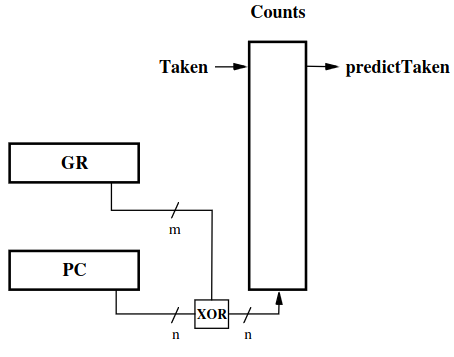
\includegraphics[width=1\textwidth]{./images/gshareDiagram.png}
                    \caption{\texttt{gshare} predictor taken from \emph{McFarling} \cite{mcfarling}}
                    \label{gshareDiagram} 
                \end{subfigure} & 
                \begin{subfigure}{0.5\textwidth}
                    \centering
                    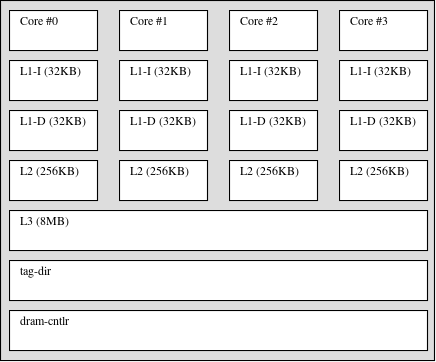
\includegraphics[width=1\textwidth]{./images/topo.png}
                    \caption{Topology for all five benchmark tests where only the number of PHT index bits was varied (all cache sizes remained consistent through every simulation). All benchmarks were run in \texttt{Sniper-7.3} with the \texttt{gainestown} configuration using the \texttt{--viz} and \texttt{--roi} options.}
                    \label{topology} 
                \end{subfigure}
            \end{tabular}
            \caption{}
            \label{intro-figures}
        \end{figure}

    \clearpage
    %%%%%%%%%%%%%%%%%%%%%%%%%%%%%%%%%%%%%%%%%%%%%%%%%%%%%%%%%%%%%%%%%%%%%%%%
    

    \section{Experimental Setup}
    \label{sec:setup}
        Simulations ran for an x86 architecture simulator, Sniper 7.3 \cite{sniper}. Since this experiment looked to sweep the \texttt{gshare} branch predictor performance through PHT sizes, each simulation is configured with the same topology (Figure \ref{topology}). The same default configurations were set in \texttt{gainestown.cfg}. 

        Three PHT sizes were swept for simulations using the \texttt{gshare} branch predictor, $2^4, 2^8, 2^{16}$. The sweep for ``size'' $2^0$ represents simulations that ran the default branch predictor, \texttt{pentium}. \texttt{gshare} was implemented separately according to technical specifications \cite{mcfarling} in C++, and integrated into \texttt{Sniper-7.3} with \texttt{gcc-7.4.0}. There was a total of 26 simulations (see Table \ref{table:configurations}). The different branch predictor configurations were simulated with five \texttt{splash2} benchmarks not previously used: \texttt{cholesky}, \texttt{lu.cont}, \texttt{radiosity}, \texttt{raytrace}, and \texttt{fmm} \cite{splash2}. 
        % \clearpage


        The workloads are briefly described as follows:

        \begin{description}
            \item[\textbf{cholesky}]: The \texttt{cholesky} factors a sparse matrix into the product of a lower triangular matrix and its transpose without globally synchronizing between steps. 
            
            
            
            \item[\textbf{fmm}]: The \texttt{fmm} application implements the adaptive Fast Multipole Method to simulate interactions of systems of N-bodies (particles, galaxies, etc.) in 2D with unstructured communication patterns.
            
            
            \item[\textbf{lu.cont}]: The \texttt{lu.cont} factors a dense matrix into the product of a lower and upper triangular matrix, exploiting temporal locality on submatrix elements. Blocks are allocated sequentially and locally to processors that own them in order to improve the spatial locality. 
            
            
            \item[\textbf{radiosity}]: The \texttt{radiosity} application computes the equilibrium distribution of light in a scene using the iterative hierarchical diffuse radiosity method using the light transport interactions and subdivisions in polygons. This application has highly irregular computation structure and data structure accesses.  
            
            \item[\textbf{raytrace}]: The \texttt{raytrace} renders a 3D scene using ray tracing through each pixel in the image plane, reflecting them off objects in unpredictable and multiple ways; therefore, data structure access patterns are also unpredictable.
        \end{description}


        All the simulations ran concurrently using bash script(s) and GNU \texttt{parallel} shell tool \cite{parallel}, and post-processing of the data were handled with python (v2.7) and bash scripts (included separately). Simulations ran on a python virtual environment and in a detached \texttt{tmux} session, due to long duration of the experiments. Sniper provided data processing tools used were: \texttt{gen\_topology.py}, \texttt{cpi-stack.py}, and \texttt{mcpat.py}. 

    \clearpage
    %%%%%%%%%%%%%%%%%%%%%%%%%%%%%%%%%%%%%%%%%%%%%%%%%%%%%%%%%%%%%%%%%%%%%%%%

    \section{Results \& Analysis}


        \subsection{Performance Analysis} %%%%%%%%%%%%%
        \label{sec:performance}

        \begin{figure}[hbt!] 
            \centering 
            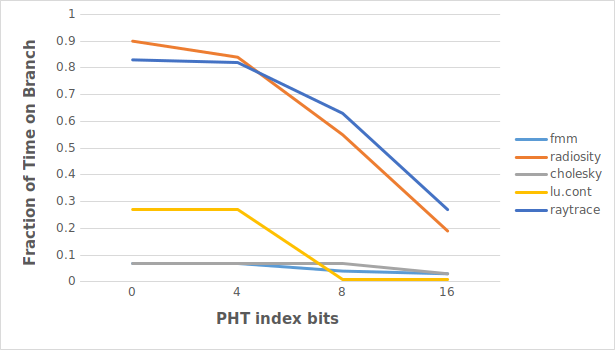
\includegraphics[width=0.8\textwidth]{images/PHTvsBranch.png}
            \caption{CPI Stack Result - Fraction of time spent on branches. As time decreases, less time is spent handling branches, including mispredictions. (See Figures \ref{appfig:cpi:cholesky}, \ref{appfig:cpi:fmm}, \ref{appfig:cpi:lu.cont}, \ref{appfig:cpi:radiosity}, and \ref{appfig:cpi:raytrace} for correlating CPI stacks.)}
            \label{fig:BRANCH}  
        \end{figure}

        For most workloads, as size of the PHT table increased, time spent on branch instructions noticeably decreases (Figure \ref{fig:BRANCH}). \texttt{fmm} and \texttt{cholesky} have less noticeable reductions because those implementations introduced less control hazards. \texttt{radiosity} and \texttt{raytrace} see more noticeable reduction due to their irregular and unpredictable access patterns more affected by branches; while \texttt{lu.cont} has less control hazards to begin with, it even sees about 96\% less time spent on branches at the highest PHT size swept compared to the default. The reduced fraction of time spent on branches indicates less time incurring cost of misprediction penalties, likely as branching information became more refined with more branch histories to inform branch decisions. 

        Reducing time on branching correlates with performance gains seen through increased IPC (Figure \ref{fig:IPC}) and reduced execution time (Figure \ref{fig:time}). With less branch misses, more correctly speculated instructions are put on the execution path, leading to more instruction executed and retired in a cycle. Without time spent recovering from control hazards, it also makes sense that the applications also run faster. These suggest that misprediction penalties contribute to a significant portion of performance loss across the five workloads, but are positively impacted by \texttt{gshare} with more global history. 


        

        \clearpage

        \begin{figure}[hbt!] 
            \centering 
            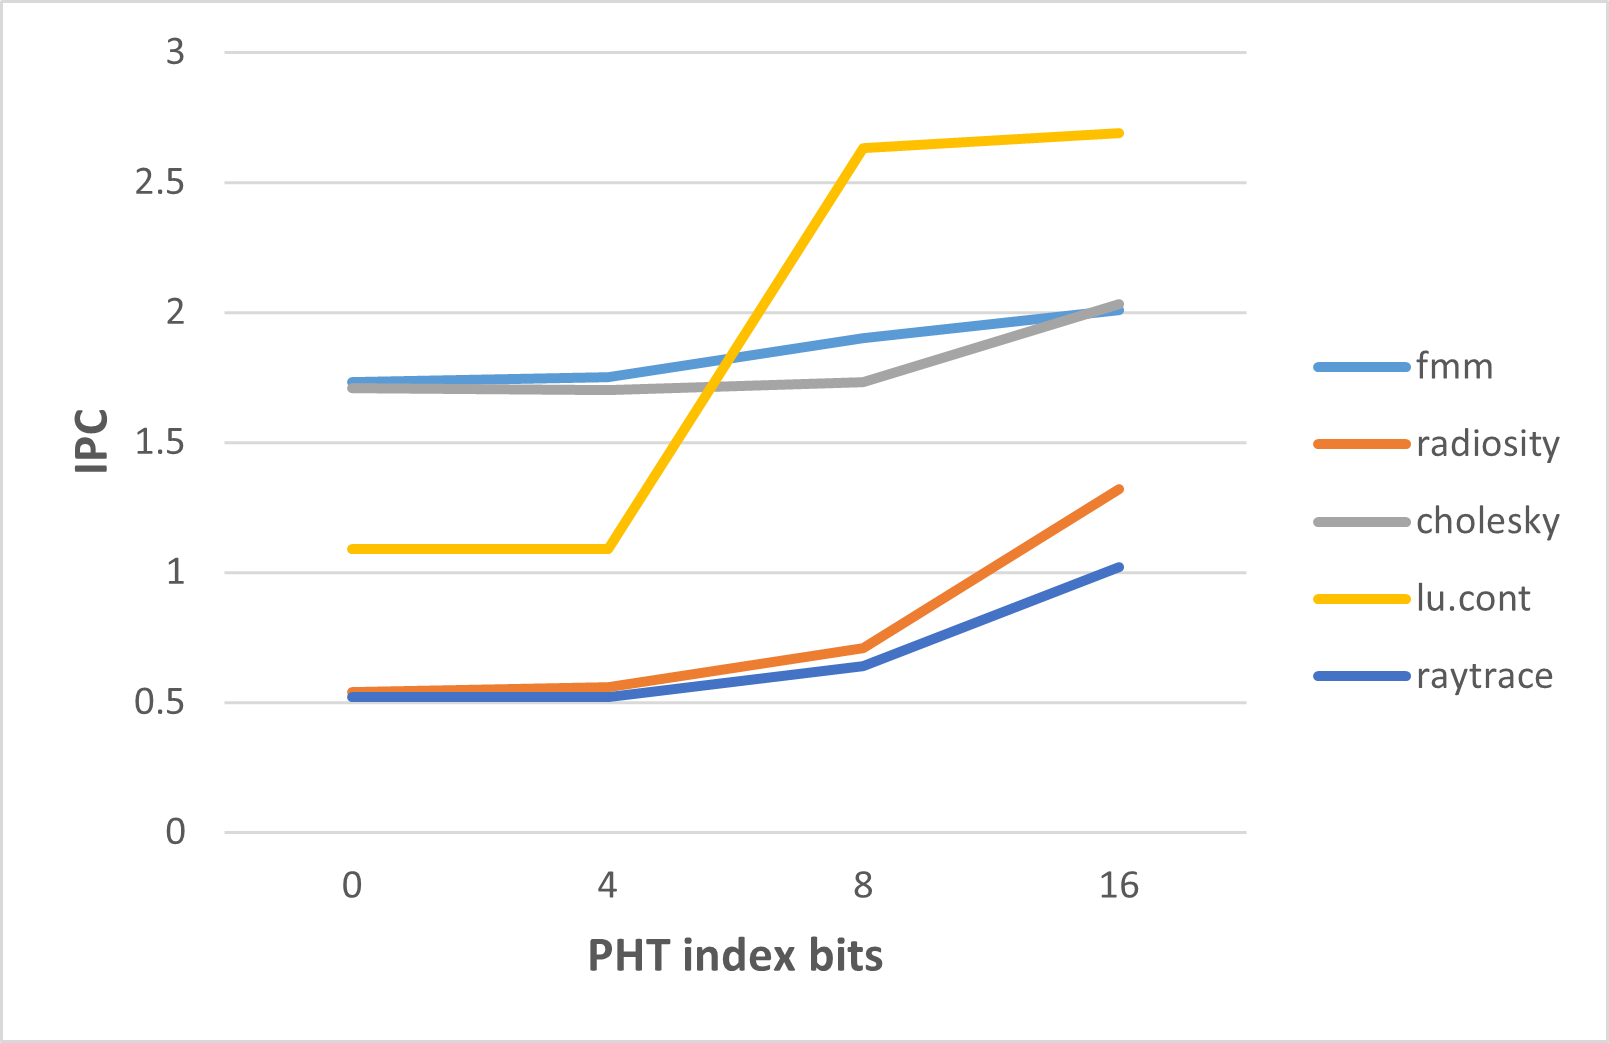
\includegraphics[width=0.8\textwidth]{images/PHTvsIPC.png}
            \caption{IPC across PHT size sweep for five benchmars. IPC increases for four sweeps and plateaus around 16 PHT index bits for \texttt{lu.cont}. (\emph{See attached all.csv file for specific data values.})}
            \label{fig:IPC} 
        \end{figure}

        \begin{figure}[hbt!]   
            \centering
            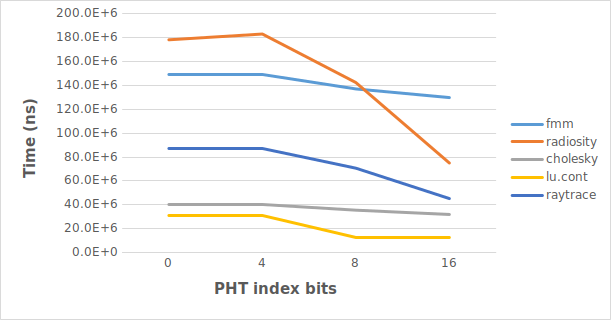
\includegraphics[width=0.8\textwidth]{images/PHTvsTime.png}
            \caption{Execution time across PHT size sweep for five benchmarks.}
            \label{fig:time} 
        \end{figure}

            

            % \textbf{No ILP benefits from OOO:} For workloads likely to not have many dependencies and implemented with little to no parallelism, they see little to no benefits in increasing the number of RS'. 
        \clearpage
        %%%%%%%%%%%%%%%%%%%%%%%%%%%%%%%%%%%%%%%%%%%%%%%%%%%%



        \subsection{Energy Consumption} %%%%%%%%%%%%%

            Peak dynamic processor power increases for the sweep across all benchmarks (Figure \ref{fig:peak-dynamic-power}). This is likely due not only to the complexity of the individual applications, but also the implementation of the integrated \texttt{gshare}, as well as the total increasing bits in a PHT. However, overall power consumption typically decreases with increasing PHT size across the five workloads (Figures \ref{appfig:power:cholesky}, \ref{appfig:power:fmm}, \ref{appfig:power:lu.cont}, \ref{appfig:power:radiosity}, and \ref{appfig:power:raytrace}). Along with faster execution time across all sweeps (Figure \ref{fig:time}), this gives a decreasing trend of EDP with the sweep, as evident by the results plotted in Figure \ref{fig:normalized-EDP}. The lower EDPs show a positive relationship between the performance and energy efficiency tradeoffs due to refining branch histories in \texttt{gshare}. Once again, this indicates the significant impact of branch penalties on a system. 

            \begin{figure}[hbt!] 
                \centering
                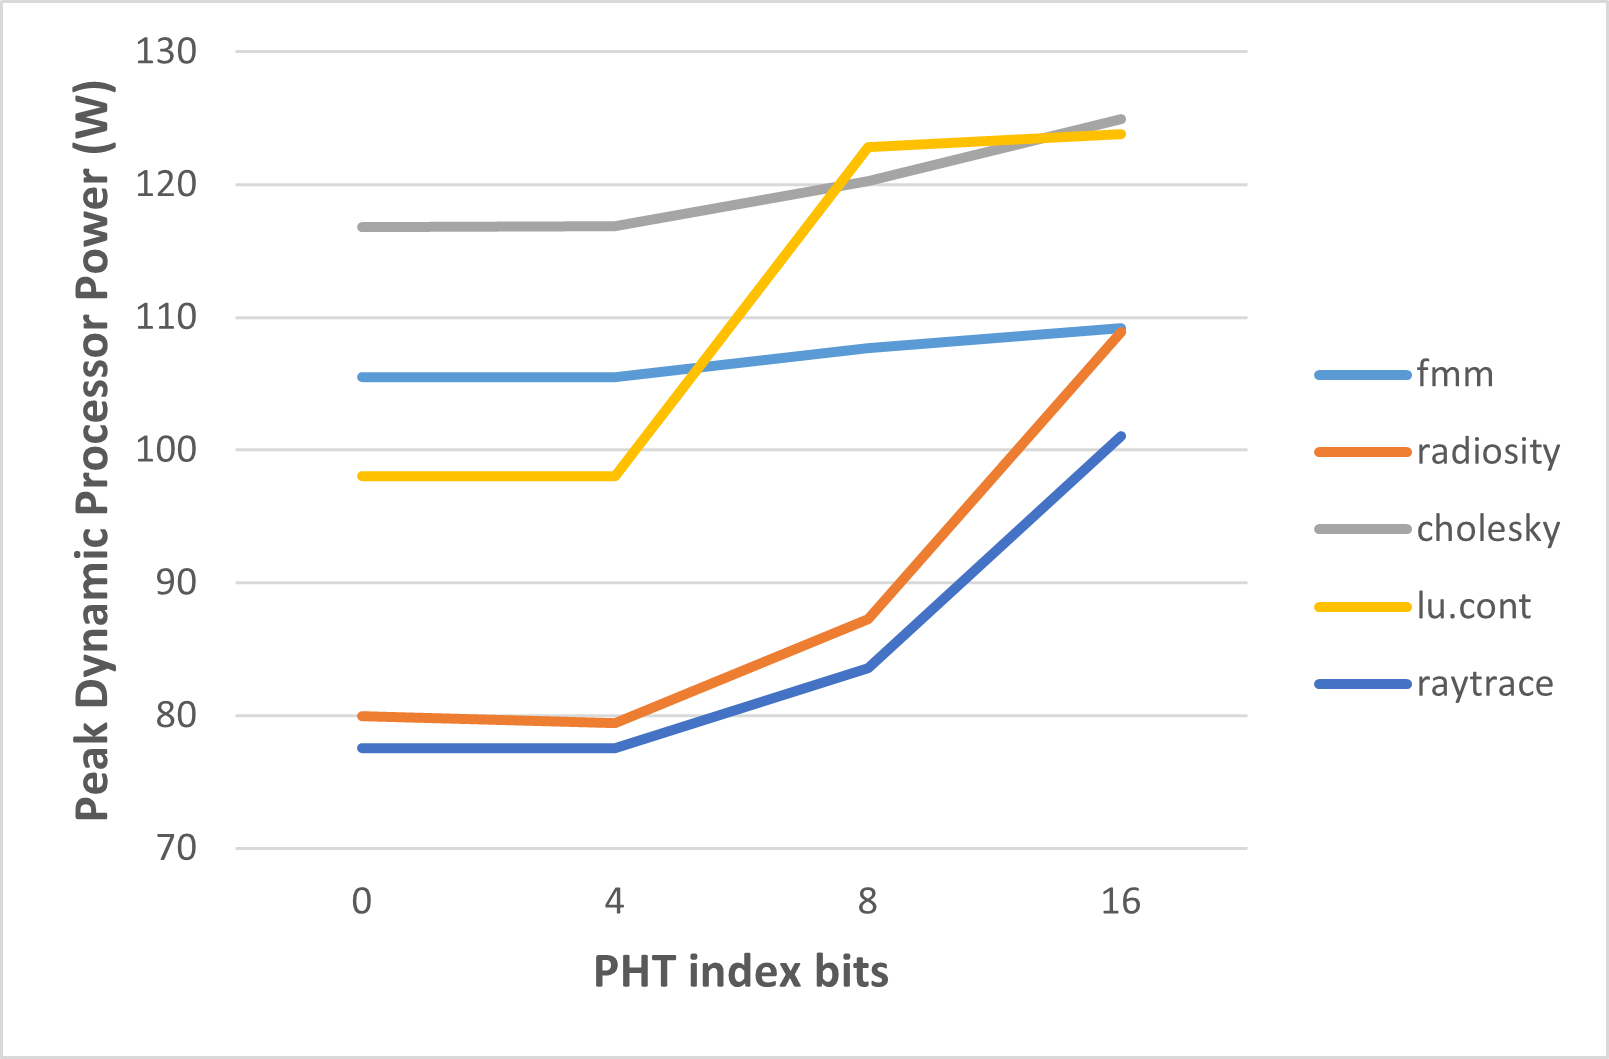
\includegraphics[width=0.8\textwidth]{images/PHTvsPower.png}
                \caption{Peak dynamic processor power across PHT size sweep for five benchmarks. Peak dynamic power continues to increase for \texttt{radiosity} and \texttt{raytrace} at the max for this work, it only slowly increases for \texttt{cholesky} and \texttt{fmm}, and plateaus for \texttt{lu.cont} around 8 to 16 PHT index bits.}
                \label{fig:peak-dynamic-power} 
            \end{figure} 

            \clearpage

            \begin{figure}[hbt!]   
                \centering
                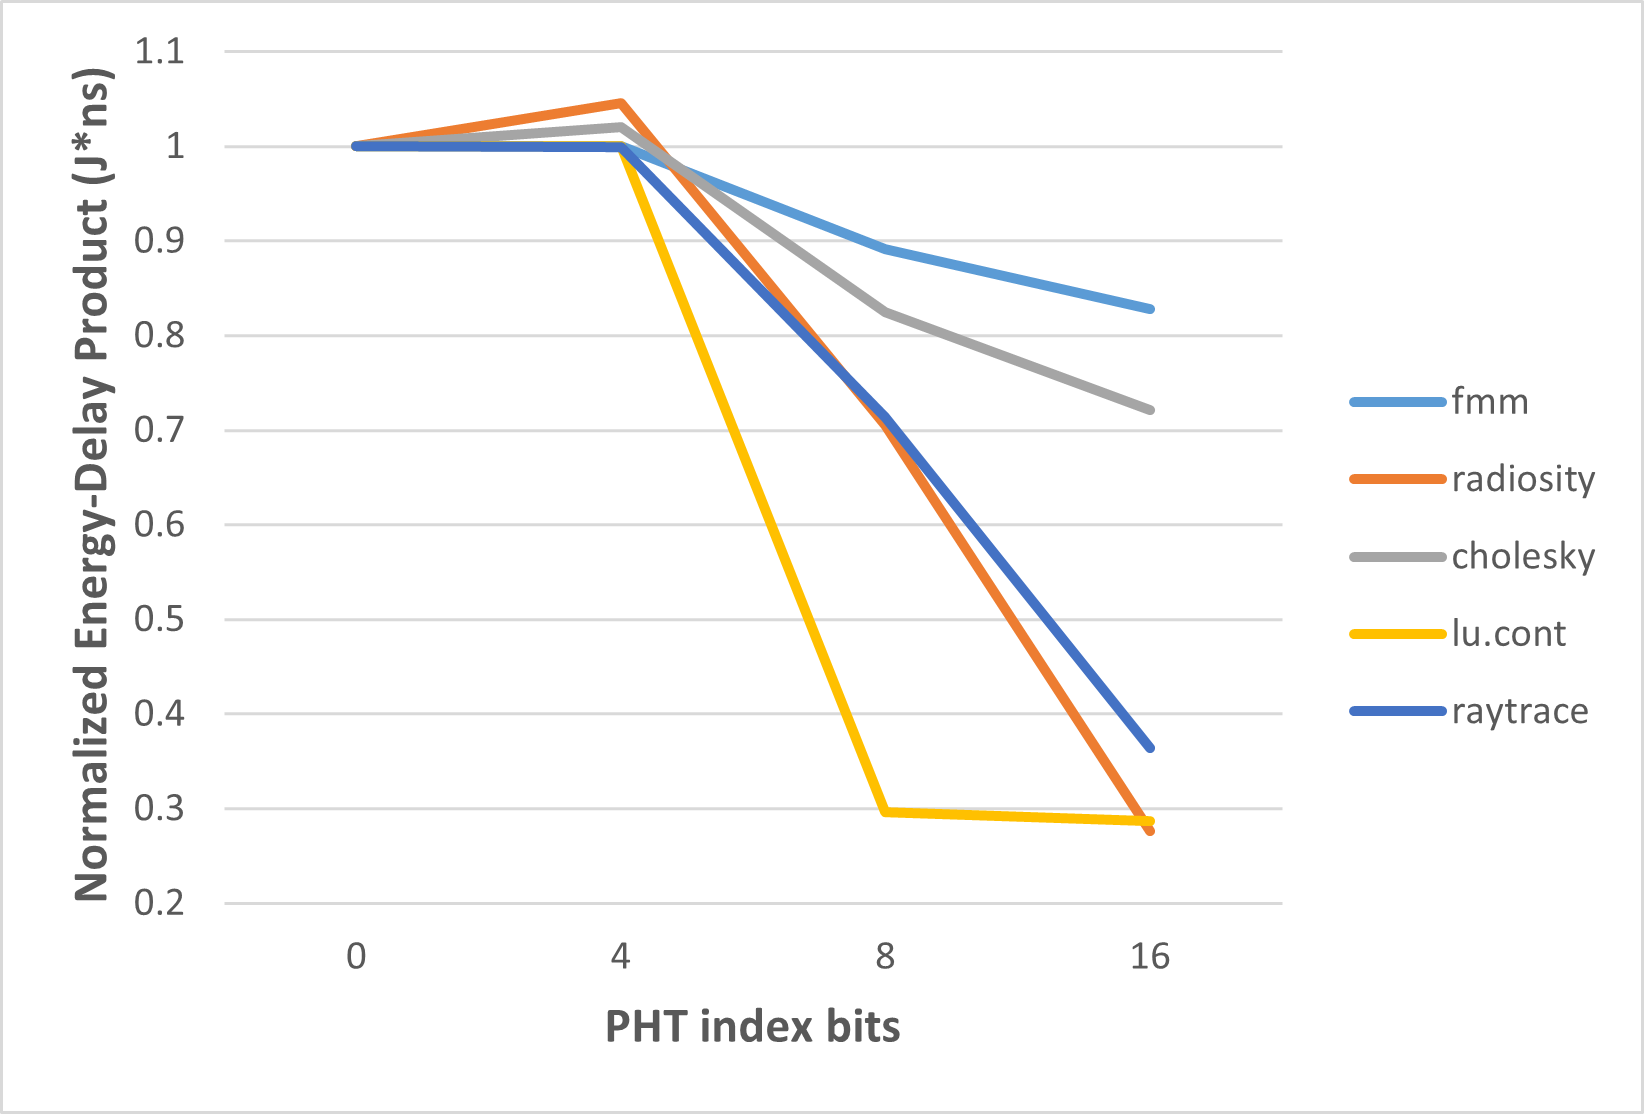
\includegraphics[width=0.8\textwidth]{images/PHTvsnEDP.png}
                \caption{Normalized energy-delay-product (EDP) across PHT size sweep for five benchmarks. EDP is given by the energy consumption (in Joules) times the execution time of the application (in nanoseconds). (See Figures \ref{appfig:power:cholesky}, \ref{appfig:power:fmm}, \ref{appfig:power:lu.cont}, \ref{appfig:power:radiosity}, and \ref{appfig:power:raytrace} for correlating Power Results.)}
                \label{fig:normalized-EDP} 
            \end{figure}
    %%%%%%%%%%%%%%%%%%%%%%%%%%%%%%%%%%%%%%%%%%%%%%%%%%%%%%%%%%%%%%%%%%%%%%%%


    \section{Conclusion}
    \label{conclusion}

        
    The integrated \texttt{gshare} predictor performed better than the default, \texttt{pentium}; with increasing PHT sizes, \texttt{gshare} reduces time spent on branching, which increases overal IPC and execution time. Not only that, but incurring less misprediction penalty leads to improved energy consumption, with an overall lowering of EDP. This shows the importance of branch predictor choice and design in overall performance. These results also suggest several obvious direction to expand this work. Only three sizes are swept for \texttt{gshare}, which shows a trend for improved performance and energy consumption; more sizes should be swept to see if the trend continues or if an optimal range for PHT size exists, after which point performance and/or energy degrades. Along with PHT size, other elements that could be examined are the number of bits in the global history register and the counter bits, as those could also refine \texttt{gshare} performance to a point. In addition, other factors of interest include comparing \texttt{gshare} against other correlating predictors, dynamic predictors, and static ones because \texttt{gshare} is already known to work well and is used as a baseline for other predictors \cite{book}, but not necessarily the optimal predictor for all types of workloads. 

    \clearpage
    %%%%%%%%%%%%%%%%%%%%%%%%%%%%%%%%%%%%%%%%%%%%%%%%%%%%%%%%%%%%%%%%%%%%%%%%

    \section{Appendix: Raw Post Processed Data}
    \label{appendix:raw}

    \subsection{cholesky} %%%%%%%%%%%%%%%%%%%%%%%%%%%%%%%%%%%
        \subsubsection{Power Results} %%%%%%%%%%%%%%%%%%%%%%%%%%%%%%%%%%%

        %%%%%%%%%% Power GRAPH %%%%%%%%%%
        \begin{figure}[hbt!]
            \centering
            \noindent\begin{subfigure}{1\textwidth}
            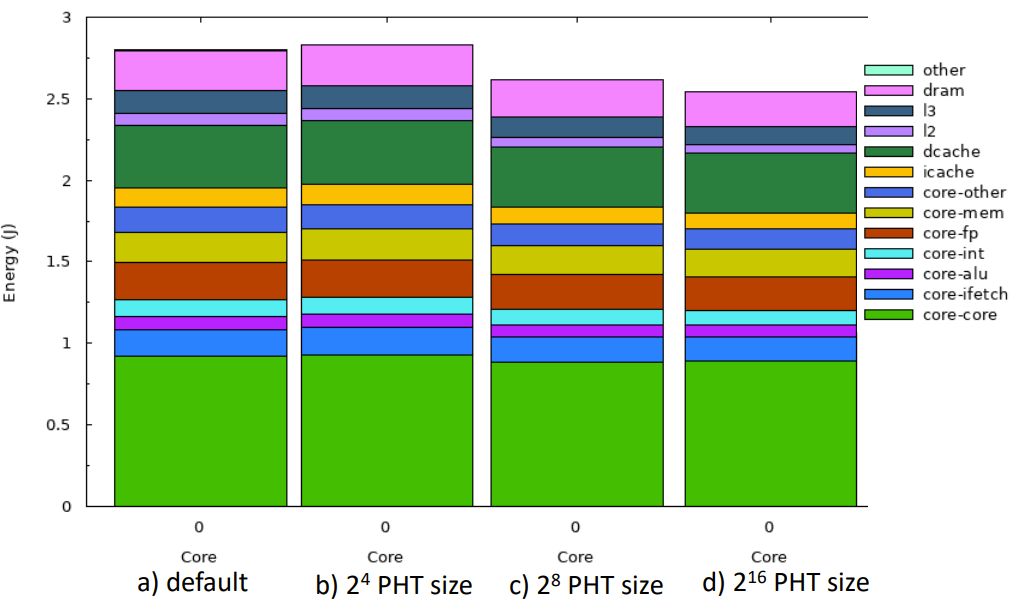
\includegraphics[width=1\textwidth]{images/Power/cholesky.PNG}
            % \caption{}
            \end{subfigure}%

            \caption{Processor power for various PHT sizes.}
            \label{appfig:power:cholesky}
        \end{figure}
        % \clearpage
        %%%%%%%%%%%%%%%%%%%%%%%%%%%%%%%%%%%

        %%%%%%%%%% Power VALUES %%%%%%%%%%
        \begin{figure}[hbt!]
            \centering
            \noindent\begin{subfigure}{0.75\textwidth}
            \lstinputlisting{../output/cholesky/0/power.out}
            \caption{default}
            \end{subfigure}%

            \noindent\begin{subfigure}{0.75\textwidth}
            \lstinputlisting{../output/cholesky/4/power.out}
            \caption{$2^{4}$ PHT size}
            \end{subfigure}%
        \end{figure}
        \clearpage

        \begin{figure}[hbt!]\ContinuedFloat
            \centering
            \noindent\begin{subfigure}{0.75\textwidth}
            \lstinputlisting{../output/cholesky/8/power.out}
            \caption{$2^{8}$ PHT size}
            \end{subfigure}%

            \noindent\begin{subfigure}{0.75\textwidth}
            \lstinputlisting{../output/cholesky/16/power.out}
            \caption{$2^{16}$ PHT size}
            \end{subfigure}%

            \caption{Specific values for each components' power consumption.}
            \label{appfig:power:cholesky:values}
        \end{figure}
        \clearpage
        %%%%%%%%%%%%%%%%%%%%%%%%%%%%%%%%%%%%%%%%%%%%%%%%%%%%%%%%%%%%%%%%%%%%%%

        \subsubsection{CPI Stacks} %%%%%%%%%%%%%%%%%%%%%%%%%%%%%%%%%%%

        %%%%%%%%%% CPI GRAPH %%%%%%%%%%
        \begin{figure}[hbt!]
            \centering
            \noindent\begin{subfigure}{0.8\textwidth}
            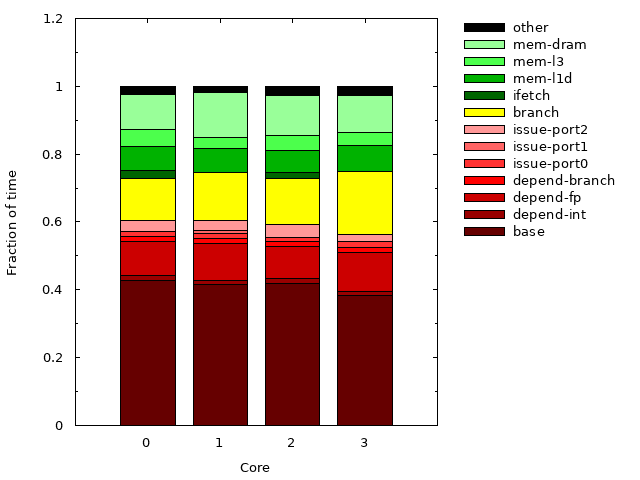
\includegraphics[width=1\textwidth]{../output/cholesky/0/cpi-stack.png}
            \caption{default}
            \end{subfigure}%

            \noindent\begin{subfigure}{0.8\textwidth}
            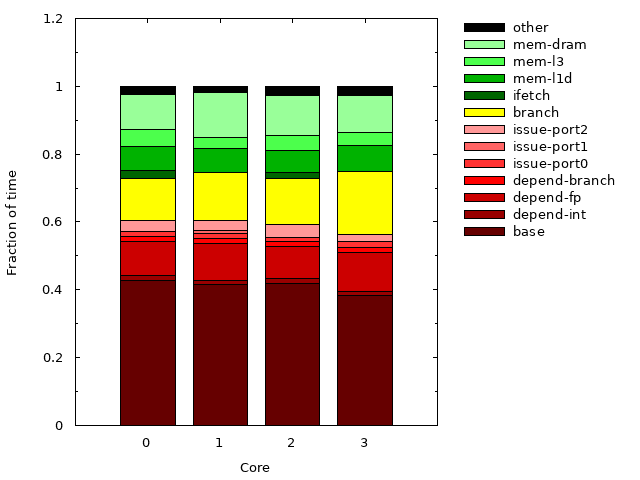
\includegraphics[width=1\textwidth]{../output/cholesky/0/cpi-stack.png}
            \caption{$2^{4}$ PHT size}
            \end{subfigure}%
        \end{figure}
        \clearpage

        \begin{figure}[hbt!]\ContinuedFloat
            \centering
            \noindent\begin{subfigure}{0.8\textwidth}
            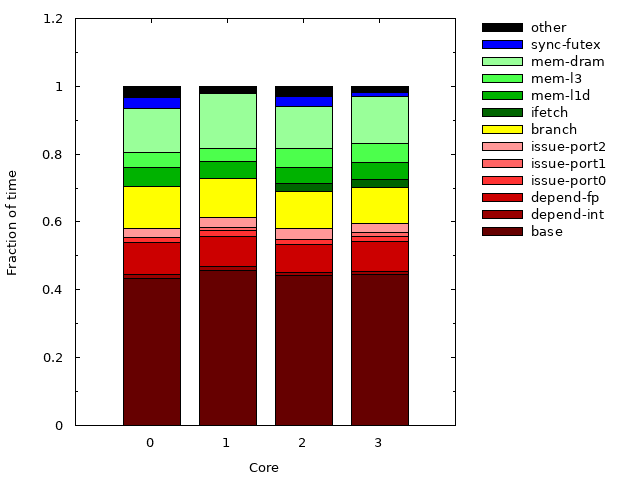
\includegraphics[width=1\textwidth]{../output/cholesky/8/cpi-stack.png}
            \caption{$2^{8}$ PHT size}
            \end{subfigure}%

            \noindent\begin{subfigure}{0.8\textwidth}
            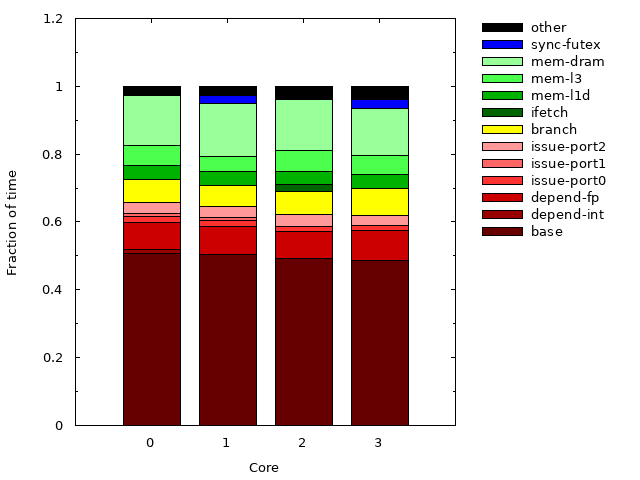
\includegraphics[width=1\textwidth]{../output/cholesky/16/cpi-stack.png}
            \caption{$2^{16}$ PHT size}
            \end{subfigure}%

            \caption{CPI stacks for various PHT sizes.}
            \label{appfig:cpi:cholesky}
        \end{figure}
        \clearpage
        %%%%%%%%%%%%%%%%%%%%%%%%%%%%%%%%%%%

        %%%%%%%%%% CPI VALUES %%%%%%%%%%
        \begin{figure}[hbt!]
            \centering
            \noindent\begin{subfigure}{0.75\textwidth}
            \lstinputlisting{../output/cholesky/0/cpi-stack.out}
            \caption{default}
            \end{subfigure}%

            \noindent\begin{subfigure}{0.75\textwidth}
            \lstinputlisting{../output/cholesky/4/cpi-stack.out}
            \caption{$2^{4}$ PHT size}
            \end{subfigure}%
        \end{figure}
        \clearpage

        \begin{figure}[hbt!]\ContinuedFloat
            \centering
            \noindent\begin{subfigure}{0.75\textwidth}
            \lstinputlisting{../output/cholesky/8/cpi-stack.out}
            \caption{$2^{8}$ PHT size}
            \end{subfigure}%

            \noindent\begin{subfigure}{0.75\textwidth}
            \lstinputlisting{../output/cholesky/16/cpi-stack.out}
            \caption{$2^{16}$ PHT size}
            \end{subfigure}%

            \caption{Specific values for each components' CPI stack.}
            \label{appfig:cpi:cholesky:values}
        \end{figure}
        \clearpage

        %%%%%%%%%%%%%%%%%%%%%%%%%%%%%%%%%%%%%%%%%%%%%%%%%%%%%%%%%%%%%%%%%%%%%%

    \subsection{fmm} %%%%%%%%%%%%%%%%%%%%%%%%%%%%%%%%%%%
        \subsubsection{Power Results} %%%%%%%%%%%%%%%%%%%%%%%%%%%%%%%%%%%

        %%%%%%%%%% Power GRAPH %%%%%%%%%%
        \begin{figure}[hbt!]
            \centering
            \noindent\begin{subfigure}{1\textwidth}
            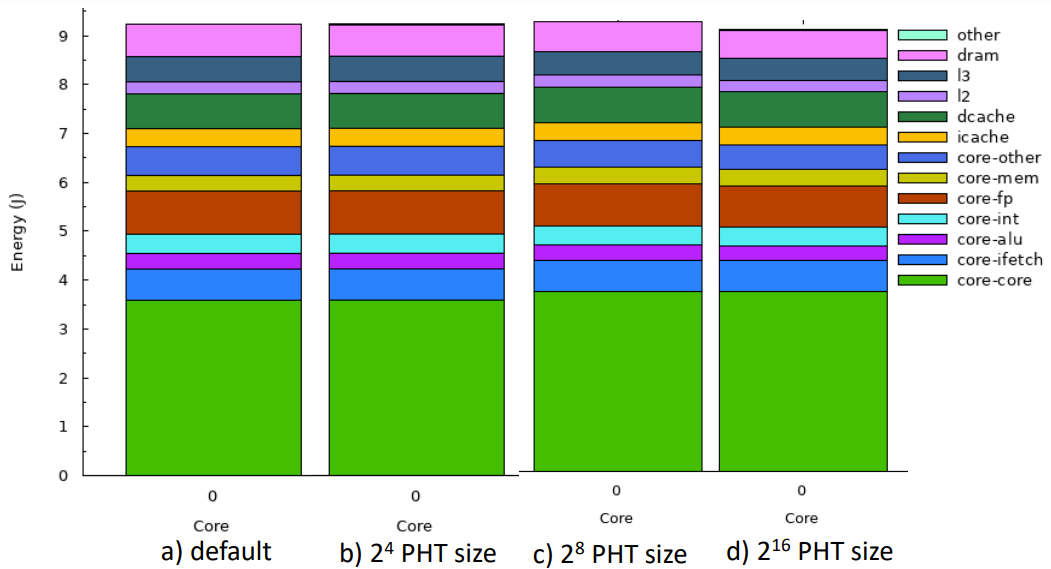
\includegraphics[width=1\textwidth]{images/Power/fmm.PNG}
            % \caption{}
            \end{subfigure}%

            \caption{Processor power for various PHT sizes.}
            \label{appfig:power:fmm}
        \end{figure}
        % \clearpage
        %%%%%%%%%%%%%%%%%%%%%%%%%%%%%%%%%%%

        %%%%%%%%%% Power VALUES %%%%%%%%%%
        \begin{figure}[hbt!]
            \centering
            \noindent\begin{subfigure}{0.75\textwidth}
            \lstinputlisting{../output/fmm/0/power.out}
            \caption{default}
            \end{subfigure}%

            \noindent\begin{subfigure}{0.75\textwidth}
            \lstinputlisting{../output/fmm/4/power.out}
            \caption{$2^{4}$ PHT size}
            \end{subfigure}%
        \end{figure}
        \clearpage

        \begin{figure}[hbt!]\ContinuedFloat
            \centering
            \noindent\begin{subfigure}{0.75\textwidth}
            \lstinputlisting{../output/fmm/8/power.out}
            \caption{$2^{8}$ PHT size}
            \end{subfigure}%

            \noindent\begin{subfigure}{0.75\textwidth}
            \lstinputlisting{../output/fmm/16/power.out}
            \caption{$2^{16}$ PHT size}
            \end{subfigure}%

            \caption{Specific values for each components' power consumption.}
            \label{appfig:power:fmm:values}
        \end{figure}
        \clearpage
        %%%%%%%%%%%%%%%%%%%%%%%%%%%%%%%%%%%%%%%%%%%%%%%%%%%%%%%%%%%%%%%%%%%%%%

        \subsubsection{CPI Stacks} %%%%%%%%%%%%%%%%%%%%%%%%%%%%%%%%%%%

        %%%%%%%%%% CPI GRAPH %%%%%%%%%%
        \begin{figure}[hbt!]
            \centering
            \noindent\begin{subfigure}{0.8\textwidth}
            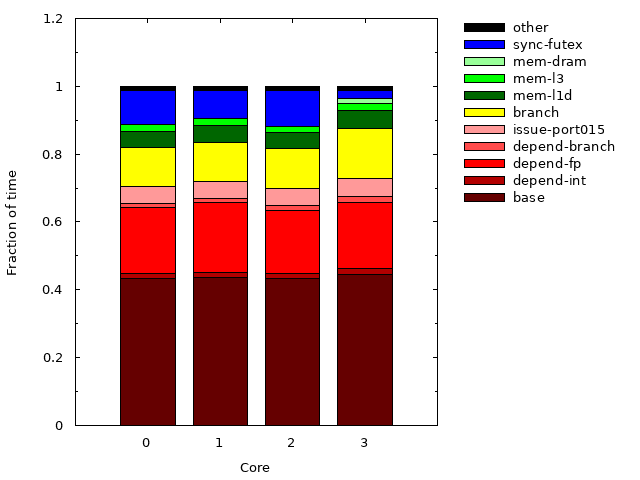
\includegraphics[width=1\textwidth]{../output/fmm/0/cpi-stack.png}
            \caption{default}
            \end{subfigure}%

            \noindent\begin{subfigure}{0.8\textwidth}
            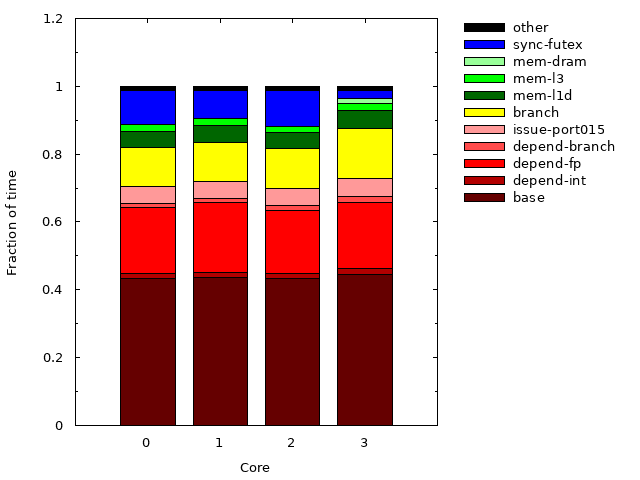
\includegraphics[width=1\textwidth]{../output/fmm/0/cpi-stack.png}
            \caption{$2^{4}$ PHT size}
            \end{subfigure}%
        \end{figure}
        \clearpage

        \begin{figure}[hbt!]\ContinuedFloat
            \centering
            \noindent\begin{subfigure}{0.8\textwidth}
            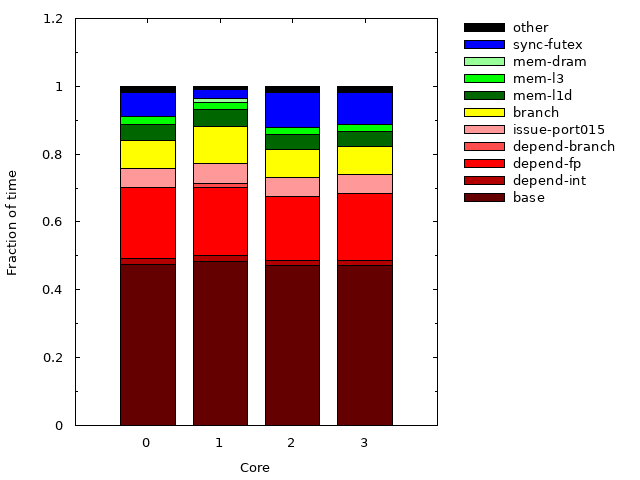
\includegraphics[width=1\textwidth]{../output/fmm/8/cpi-stack.png}
            \caption{$2^{8}$ PHT size}
            \end{subfigure}%

            \noindent\begin{subfigure}{0.8\textwidth}
            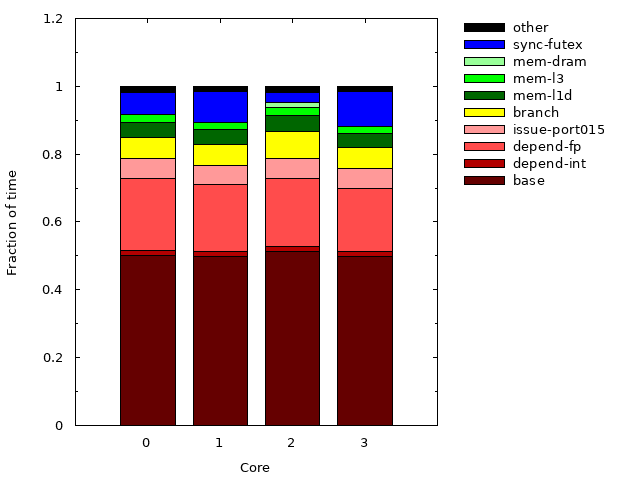
\includegraphics[width=1\textwidth]{../output/fmm/16/cpi-stack.png}
            \caption{$2^{16}$ PHT size}
            \end{subfigure}%

            \caption{CPI stacks for various PHT sizes.}
            \label{appfig:cpi:fmm}
        \end{figure}
        \clearpage
        %%%%%%%%%%%%%%%%%%%%%%%%%%%%%%%%%%%

        %%%%%%%%%% CPI VALUES %%%%%%%%%%
        \begin{figure}[hbt!]
            \centering
            \noindent\begin{subfigure}{0.75\textwidth}
            \lstinputlisting{../output/fmm/0/cpi-stack.out}
            \caption{default}
            \end{subfigure}%

            \noindent\begin{subfigure}{0.75\textwidth}
            \lstinputlisting{../output/fmm/4/cpi-stack.out}
            \caption{$2^{4}$ PHT size}
            \end{subfigure}%
        \end{figure}
        \clearpage

        \begin{figure}[hbt!]\ContinuedFloat
            \centering
            \noindent\begin{subfigure}{0.75\textwidth}
            \lstinputlisting{../output/fmm/8/cpi-stack.out}
            \caption{$2^{8}$ PHT size}
            \end{subfigure}%

            \noindent\begin{subfigure}{0.75\textwidth}
            \lstinputlisting{../output/fmm/16/cpi-stack.out}
            \caption{$2^{16}$ PHT size}
            \end{subfigure}%

            \caption{Specific values for each components' CPI stack.}
            \label{appfig:cpi:fmm:values}
        \end{figure}
        \clearpage
        %%%%%%%%%%%%%%%%%%%%%%%%%%%%%%%%%%%%%%%%%%%%%%%%%%%%%%%%%%%%%%%%%%%%%%

    \subsection{lu.cont} %%%%%%%%%%%%%%%%%%%%%%%%%%%%%%%%%%%
        \subsubsection{Power Results} %%%%%%%%%%%%%%%%%%%%%%%%%%%%%%%%%%%

        %%%%%%%%%% Power GRAPH %%%%%%%%%%
        \begin{figure}[hbt!]
            \centering
            \noindent\begin{subfigure}{1\textwidth}
            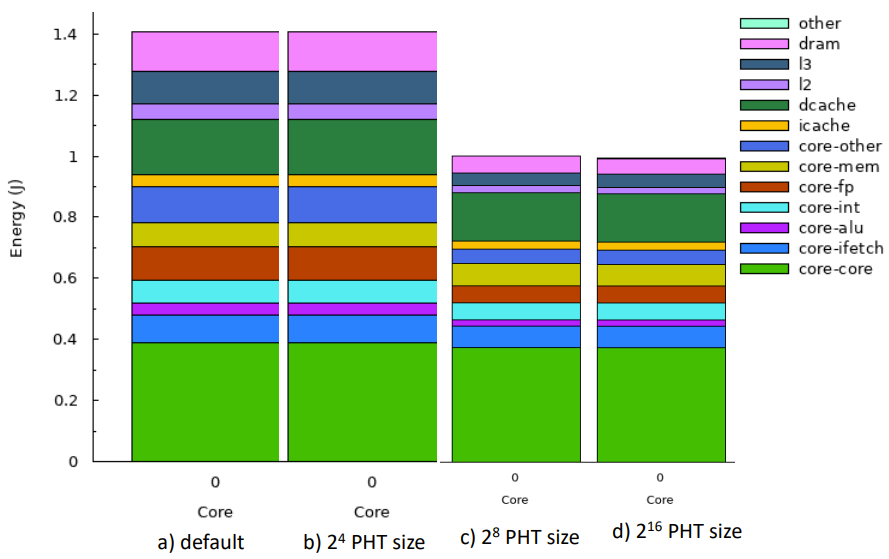
\includegraphics[width=1\textwidth]{images/Power/lu.cont.PNG}
            % \caption{}
            \end{subfigure}%

            \caption{Processor power for various PHT sizes.}
            \label{appfig:power:lu.cont}
        \end{figure}
        % \clearpage
        %%%%%%%%%%%%%%%%%%%%%%%%%%%%%%%%%%%

        %%%%%%%%%% Power VALUES %%%%%%%%%%
        \begin{figure}[hbt!]
            \centering
            \noindent\begin{subfigure}{0.75\textwidth}
            \lstinputlisting{../output/lu.cont/0/power.out}
            \caption{default}
            \end{subfigure}%

            \noindent\begin{subfigure}{0.75\textwidth}
            \lstinputlisting{../output/lu.cont/4/power.out}
            \caption{$2^{4}$ PHT size}
            \end{subfigure}%
        \end{figure}
        \clearpage

        \begin{figure}[hbt!]\ContinuedFloat
            \centering
            \noindent\begin{subfigure}{0.75\textwidth}
            \lstinputlisting{../output/lu.cont/8/power.out}
            \caption{$2^{8}$ PHT size}
            \end{subfigure}%

            \noindent\begin{subfigure}{0.75\textwidth}
            \lstinputlisting{../output/lu.cont/16/power.out}
            \caption{$2^{16}$ PHT size}
            \end{subfigure}%

            \caption{Specific values for each components' power consumption.}
            \label{appfig:power:lu.cont:values}
        \end{figure}
        \clearpage
        %%%%%%%%%%%%%%%%%%%%%%%%%%%%%%%%%%%%%%%%%%%%%%%%%%%%%%%%%%%%%%%%%%%%%%

        \subsubsection{CPI Stacks} %%%%%%%%%%%%%%%%%%%%%%%%%%%%%%%%%%%

        %%%%%%%%%% CPI GRAPH %%%%%%%%%%
        \begin{figure}[hbt!]
            \centering
            \noindent\begin{subfigure}{0.8\textwidth}
            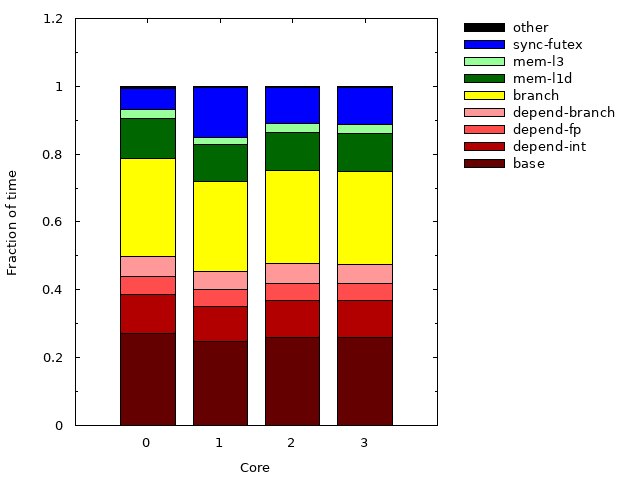
\includegraphics[width=1\textwidth]{../output/lu.cont/0/cpi-stack.png}
            \caption{default}
            \end{subfigure}%

            \noindent\begin{subfigure}{0.8\textwidth}
            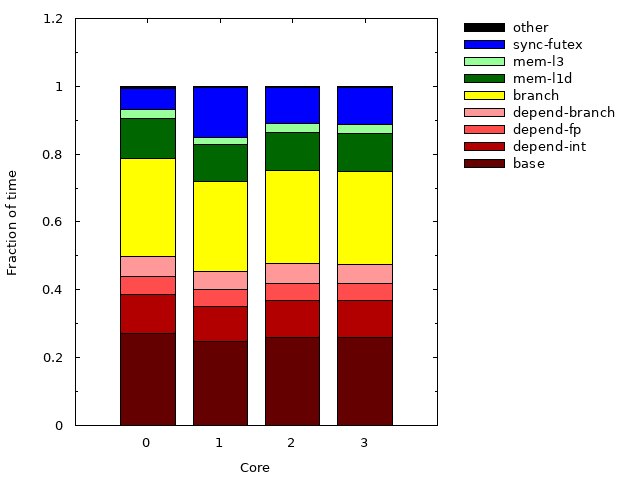
\includegraphics[width=1\textwidth]{../output/lu.cont/0/cpi-stack.png}
            \caption{$2^{4}$ PHT size}
            \end{subfigure}%
        \end{figure}
        \clearpage

        \begin{figure}[hbt!]\ContinuedFloat
            \centering
            \noindent\begin{subfigure}{0.8\textwidth}
            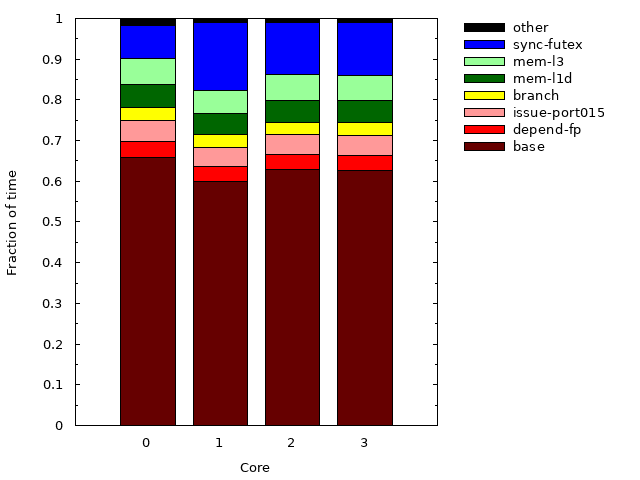
\includegraphics[width=1\textwidth]{../output/lu.cont/8/cpi-stack.png}
            \caption{$2^{8}$ PHT size}
            \end{subfigure}%

            \noindent\begin{subfigure}{0.8\textwidth}
            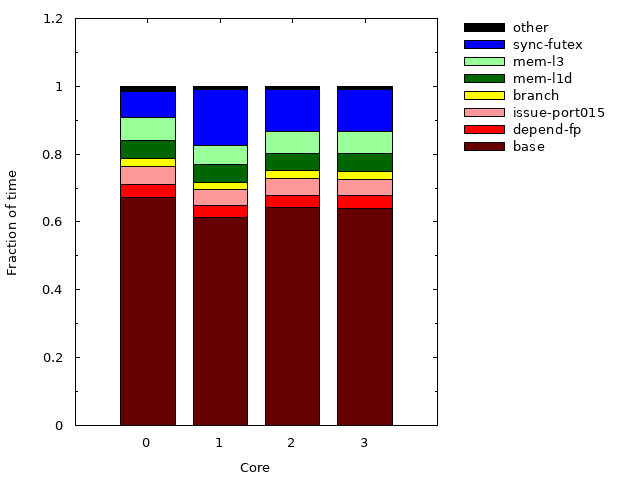
\includegraphics[width=1\textwidth]{../output/lu.cont/16/cpi-stack.png}
            \caption{$2^{16}$ PHT size}
            \end{subfigure}%

            \caption{CPI stacks for various PHT sizes.}
            \label{appfig:cpi:lu.cont}
        \end{figure}
        \clearpage
        %%%%%%%%%%%%%%%%%%%%%%%%%%%%%%%%%%%

        %%%%%%%%%% CPI VALUES %%%%%%%%%%
        \begin{figure}[hbt!]
            \centering
            \noindent\begin{subfigure}{0.75\textwidth}
            \lstinputlisting{../output/lu.cont/0/cpi-stack.out}
            \caption{default}
            \end{subfigure}%

            \noindent\begin{subfigure}{0.75\textwidth}
            \lstinputlisting{../output/lu.cont/4/cpi-stack.out}
            \caption{$2^{4}$ PHT size}
            \end{subfigure}%
        \end{figure}
        \clearpage

        \begin{figure}[hbt!]\ContinuedFloat
            \centering
            \noindent\begin{subfigure}{0.75\textwidth}
            \lstinputlisting{../output/lu.cont/8/cpi-stack.out}
            \caption{$2^{8}$ PHT size}
            \end{subfigure}%

            \noindent\begin{subfigure}{0.75\textwidth}
            \lstinputlisting{../output/lu.cont/16/cpi-stack.out}
            \caption{$2^{16}$ PHT size}
            \end{subfigure}%

            \caption{Specific values for each components' CPI stack.}
            \label{appfig:cpi:lu.cont:values}
        \end{figure}
        \clearpage
        %%%%%%%%%%%%%%%%%%%%%%%%%%%%%%%%%%%%%%%%%%%%%%%%%%%%%%%%%%%%%%%%%%%%%%

    \subsection{radiosity} %%%%%%%%%%%%%%%%%%%%%%%%%%%%%%%%%%%
        \subsubsection{Power Results} %%%%%%%%%%%%%%%%%%%%%%%%%%%%%%%%%%%

        %%%%%%%%%% Power GRAPH %%%%%%%%%%
        \begin{figure}[hbt!]
            \centering
            \noindent\begin{subfigure}{1\textwidth}
            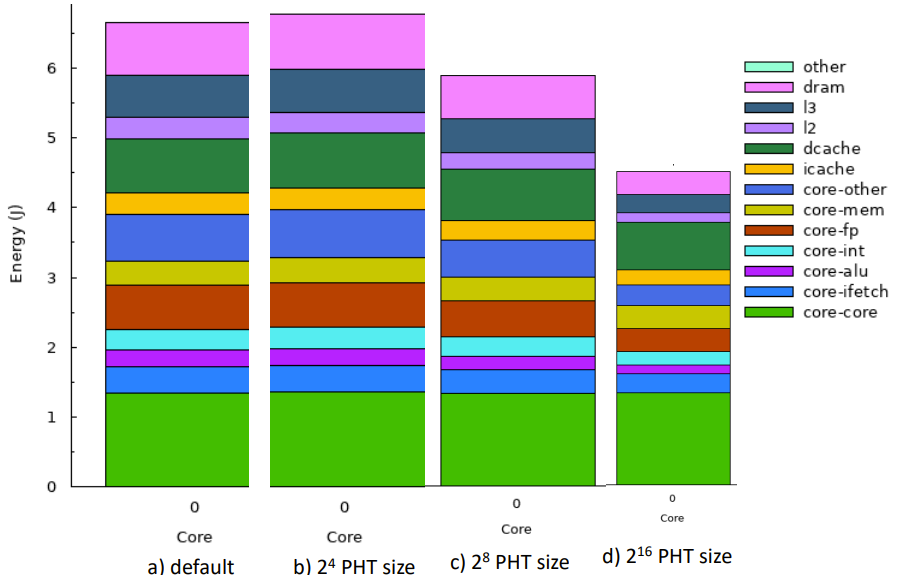
\includegraphics[width=1\textwidth]{images/Power/radiosity.PNG}
            % \caption{}
            \end{subfigure}%

            \caption{Processor power for various PHT sizes.}
            \label{appfig:power:radiosity}
        \end{figure}
        % \clearpage
        %%%%%%%%%%%%%%%%%%%%%%%%%%%%%%%%%%%

        %%%%%%%%%% Power VALUES %%%%%%%%%%
        \begin{figure}[hbt!]
            \centering
            \noindent\begin{subfigure}{0.75\textwidth}
            \lstinputlisting{../output/radiosity/0/power.out}
            \caption{default}
            \end{subfigure}%

            \noindent\begin{subfigure}{0.75\textwidth}
            \lstinputlisting{../output/radiosity/4/power.out}
            \caption{$2^{4}$ PHT size}
            \end{subfigure}%
        \end{figure}
        \clearpage

        \begin{figure}[hbt!]\ContinuedFloat
            \centering
            \noindent\begin{subfigure}{0.75\textwidth}
            \lstinputlisting{../output/radiosity/8/power.out}
            \caption{$2^{8}$ PHT size}
            \end{subfigure}%

            \noindent\begin{subfigure}{0.75\textwidth}
            \lstinputlisting{../output/radiosity/16/power.out}
            \caption{$2^{16}$ PHT size}
            \end{subfigure}%

            \caption{Specific values for each components' power consumption.}
            \label{appfig:power:radiosity:values}
        \end{figure}
        \clearpage
        %%%%%%%%%%%%%%%%%%%%%%%%%%%%%%%%%%%%%%%%%%%%%%%%%%%%%%%%%%%%%%%%%%%%%%

        \subsubsection{CPI Stacks} %%%%%%%%%%%%%%%%%%%%%%%%%%%%%%%%%%%

        %%%%%%%%%% CPI GRAPH %%%%%%%%%%
        \begin{figure}[hbt!]
            \centering
            \noindent\begin{subfigure}{0.8\textwidth}
            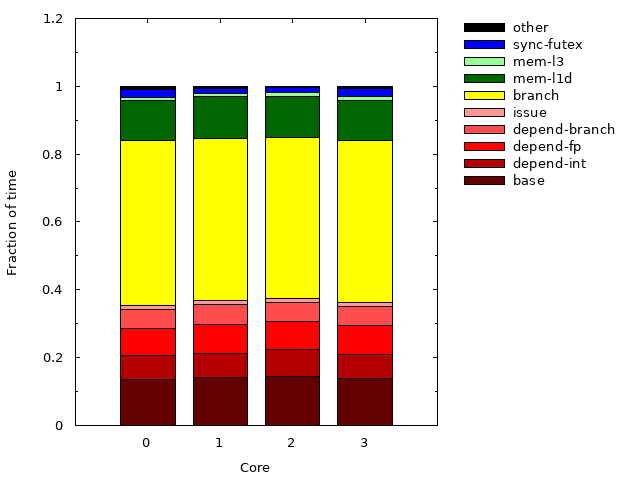
\includegraphics[width=1\textwidth]{../output/radiosity/0/cpi-stack.png}
            \caption{default}
            \end{subfigure}%

            \noindent\begin{subfigure}{0.8\textwidth}
            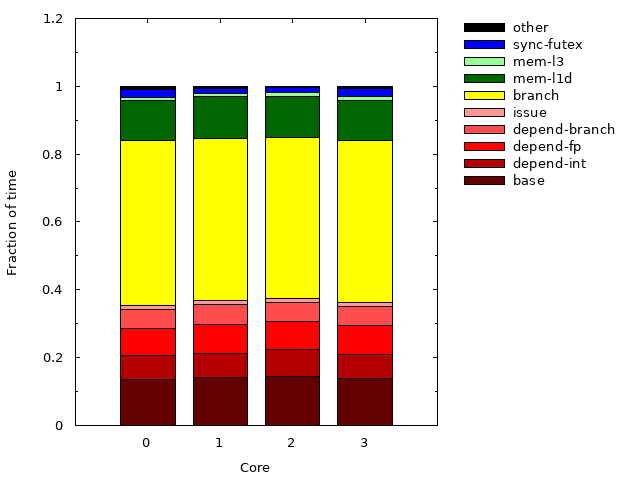
\includegraphics[width=1\textwidth]{../output/radiosity/0/cpi-stack.png}
            \caption{$2^{4}$ PHT size}
            \end{subfigure}%
        \end{figure}
        \clearpage

        \begin{figure}[hbt!]\ContinuedFloat
            \centering
            \noindent\begin{subfigure}{0.8\textwidth}
            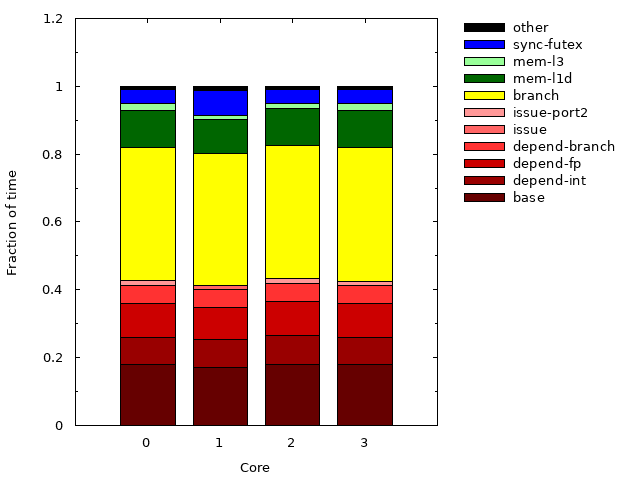
\includegraphics[width=1\textwidth]{../output/radiosity/8/cpi-stack.png}
            \caption{$2^{8}$ PHT size}
            \end{subfigure}%

            \noindent\begin{subfigure}{0.8\textwidth}
            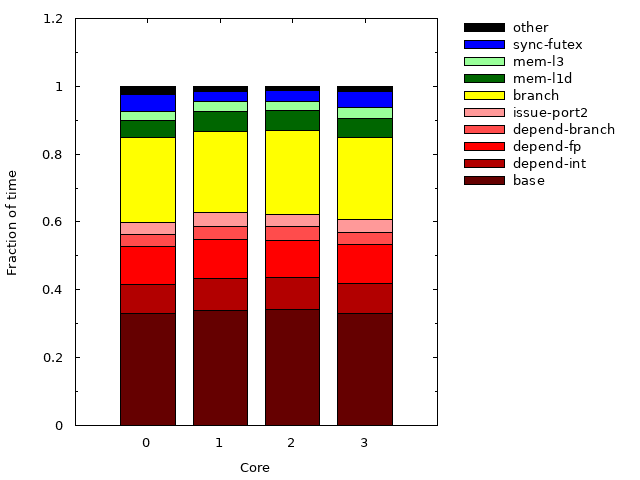
\includegraphics[width=1\textwidth]{../output/radiosity/16/cpi-stack.png}
            \caption{$2^{16}$ PHT size}
            \end{subfigure}%

            \caption{CPI stacks for various PHT sizes.}
            \label{appfig:cpi:radiosity}
        \end{figure}
        \clearpage
        %%%%%%%%%%%%%%%%%%%%%%%%%%%%%%%%%%%

        %%%%%%%%%% CPI VALUES %%%%%%%%%%
        \begin{figure}[hbt!]
            \centering
            \noindent\begin{subfigure}{0.75\textwidth}
            \lstinputlisting{../output/radiosity/0/cpi-stack.out}
            \caption{default}
            \end{subfigure}%

            \noindent\begin{subfigure}{0.75\textwidth}
            \lstinputlisting{../output/radiosity/4/cpi-stack.out}
            \caption{$2^{4}$ PHT size}
            \end{subfigure}%
        \end{figure}
        \clearpage

        \begin{figure}[hbt!]\ContinuedFloat
            \centering
            \noindent\begin{subfigure}{0.75\textwidth}
            \lstinputlisting{../output/radiosity/8/cpi-stack.out}
            \caption{$2^{8}$ PHT size}
            \end{subfigure}%

            \noindent\begin{subfigure}{0.75\textwidth}
            \lstinputlisting{../output/radiosity/16/cpi-stack.out}
            \caption{$2^{16}$ PHT size}
            \end{subfigure}%

            \caption{Specific values for each components' CPI stack.}
            \label{appfig:cpi:radiosity:values}
        \end{figure}
        \clearpage
        %%%%%%%%%%%%%%%%%%%%%%%%%%%%%%%%%%%%%%%%%%%%%%%%%%%%%%%%%%%%%%%%%%%%%%

    \subsection{raytrace} %%%%%%%%%%%%%%%%%%%%%%%%%%%%%%%%%%%
        \subsubsection{Power Results} %%%%%%%%%%%%%%%%%%%%%%%%%%%%%%%%%%%

        %%%%%%%%%% Power GRAPH %%%%%%%%%%
        \begin{figure}[hbt!]
            \centering
            \noindent\begin{subfigure}{1\textwidth}
            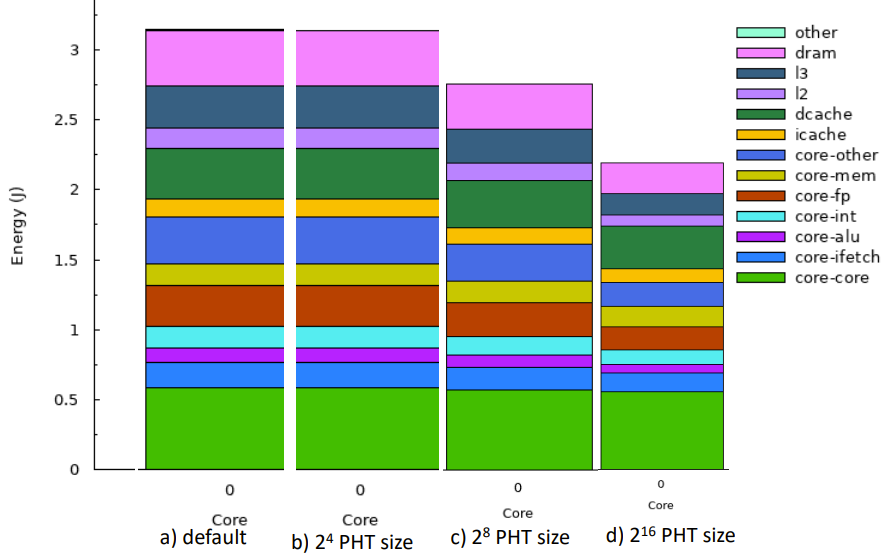
\includegraphics[width=1\textwidth]{images/Power/raytrace.PNG}
            % \caption{}
            \end{subfigure}% 

            \caption{Processor power for various PHT sizes.}
            \label{appfig:power:raytrace}
        \end{figure}
        % \clearpage
        %%%%%%%%%%%%%%%%%%%%%%%%%%%%%%%%%%%

        %%%%%%%%%% Power VALUES %%%%%%%%%%
        \begin{figure}[hbt!]
            \centering
            \noindent\begin{subfigure}{0.75\textwidth}
            \lstinputlisting{../output/raytrace/0/power.out}
            \caption{default}
            \end{subfigure}%

            \noindent\begin{subfigure}{0.75\textwidth}
            \lstinputlisting{../output/raytrace/4/power.out}
            \caption{$2^{4}$ PHT size}
            \end{subfigure}%
        \end{figure}
        \clearpage

        \begin{figure}[hbt!]\ContinuedFloat
            \centering
            \noindent\begin{subfigure}{0.75\textwidth}
            \lstinputlisting{../output/raytrace/8/power.out}
            \caption{$2^{8}$ PHT size}
            \end{subfigure}%

            \noindent\begin{subfigure}{0.75\textwidth}
            \lstinputlisting{../output/raytrace/16/power.out}
            \caption{$2^{16}$ PHT size}
            \end{subfigure}%

            \caption{Specific values for each components' power consumption.}
            \label{appfig:power:raytrace:values}
        \end{figure}
        \clearpage
        %%%%%%%%%%%%%%%%%%%%%%%%%%%%%%%%%%%%%%%%%%%%%%%%%%%%%%%%%%%%%%%%%%%%%%

        \subsubsection{CPI Stacks} %%%%%%%%%%%%%%%%%%%%%%%%%%%%%%%%%%%

        %%%%%%%%%% CPI GRAPH %%%%%%%%%%
        \begin{figure}[hbt!]
            \centering
            \noindent\begin{subfigure}{0.8\textwidth}
            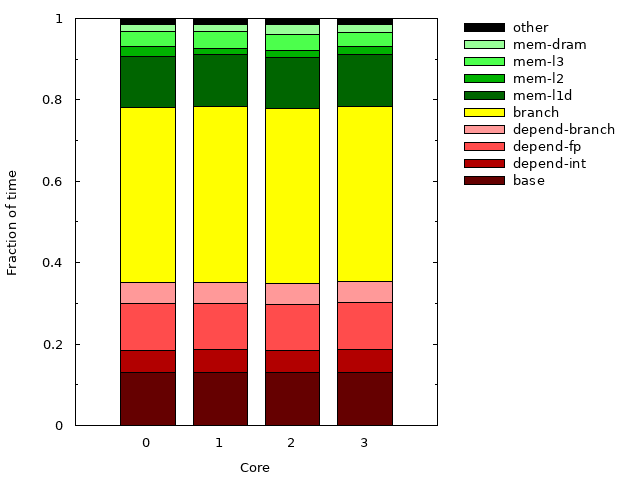
\includegraphics[width=1\textwidth]{../output/raytrace/0/cpi-stack.png}
            \caption{default}
            \end{subfigure}%

            \noindent\begin{subfigure}{0.8\textwidth}
            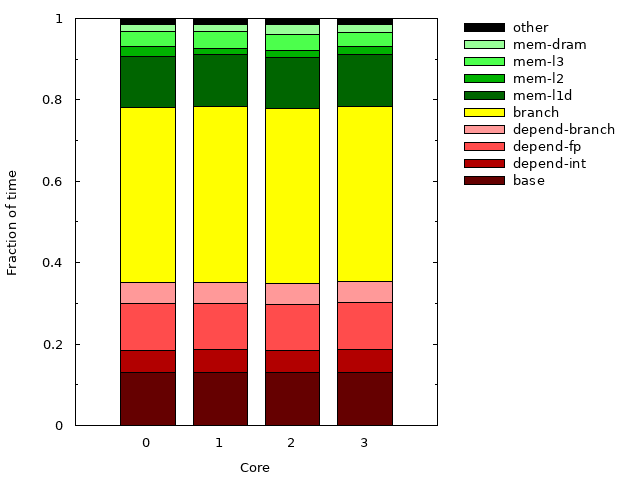
\includegraphics[width=1\textwidth]{../output/raytrace/0/cpi-stack.png}
            \caption{$2^{4}$ PHT size}
            \end{subfigure}%
        \end{figure}
        \clearpage

        \begin{figure}[hbt!]\ContinuedFloat
            \centering
            \noindent\begin{subfigure}{0.8\textwidth}
            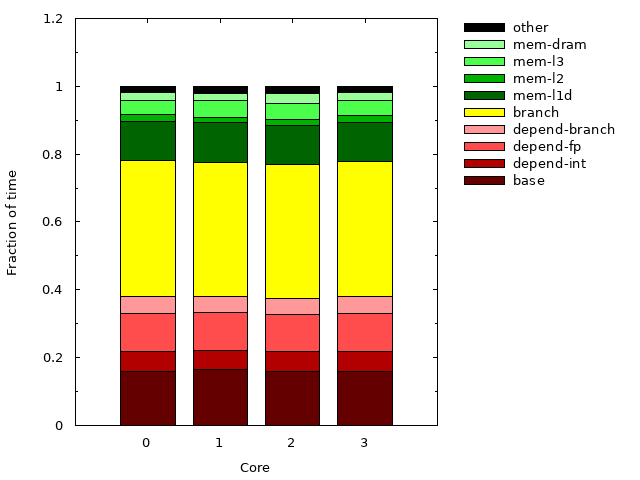
\includegraphics[width=1\textwidth]{../output/raytrace/8/cpi-stack.png}
            \caption{$2^{8}$ PHT size}
            \end{subfigure}%

            \noindent\begin{subfigure}{0.8\textwidth}
            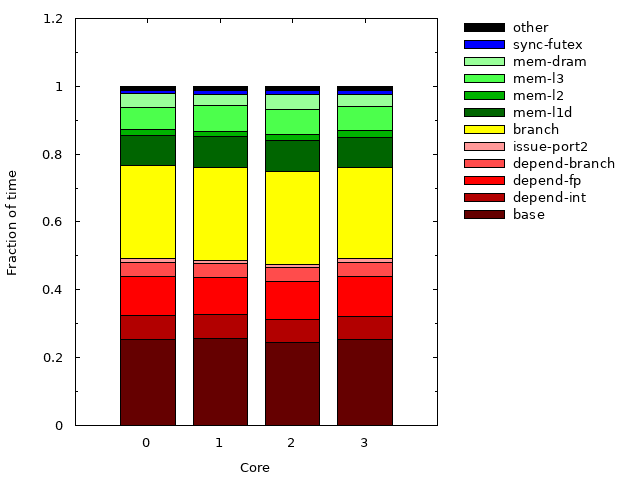
\includegraphics[width=1\textwidth]{../output/raytrace/16/cpi-stack.png}
            \caption{$2^{16}$ PHT size}
            \end{subfigure}%

            \caption{CPI stacks for various PHT sizes.}
            \label{appfig:cpi:raytrace}
        \end{figure}
        \clearpage
        %%%%%%%%%%%%%%%%%%%%%%%%%%%%%%%%%%%

        %%%%%%%%%% CPI VALUES %%%%%%%%%%
        \begin{figure}[hbt!]
            \centering
            \noindent\begin{subfigure}{0.75\textwidth}
            \lstinputlisting{../output/raytrace/0/cpi-stack.out}
            \caption{default}
            \end{subfigure}%

            \noindent\begin{subfigure}{0.75\textwidth}
            \lstinputlisting{../output/raytrace/4/cpi-stack.out}
            \caption{$2^{4}$ PHT size}
            \end{subfigure}%
        \end{figure}
        \clearpage

        \begin{figure}[hbt!]\ContinuedFloat
            \centering
            \noindent\begin{subfigure}{0.75\textwidth}
            \lstinputlisting{../output/raytrace/8/cpi-stack.out}
            \caption{$2^{8}$ PHT size}
            \end{subfigure}%

            \noindent\begin{subfigure}{0.75\textwidth}
            \lstinputlisting{../output/raytrace/16/cpi-stack.out}
            \caption{$2^{16}$ PHT size}
            \end{subfigure}%

            \caption{Specific values for each components' CPI stack.}
            \label{appfig:cpi:raytrace:values}
        \end{figure}
        \clearpage
        %%%%%%%%%%%%%%%%%%%%%%%%%%%%%%%%%%%%%%%%%%%%%%%%%%%%%%%%%%%%%%%%%%%%%%

\end{document}